\documentclass[doc]{apa}%can be jou (for journal), man (manuscript) or doc (document)

\usepackage{thumbpdf, amssymb, amsmath, amsthm, microtype,
	    graphicx, verbatim, listings, color, fancybox}
\usepackage[pdftex]{hyperref}
%\usepackage[margin=1in]{geometry}
\usepackage{cawsty}
\usepackage{fullpage}
\usepackage{pseudocode}

\usepackage{algorithm}
%\usepackage{algorithmic}
\usepackage{amsmath}
\usepackage{amsthm}
\usepackage{algpseudocode}
\usepackage{algorithmicx}% http://ctan.org/pkg/algorithmicx
\usepackage{lipsum}% http://ctan.org/pkg/lipsum
\usepackage{xifthen}% http://ctan.org/pkg/xifthen
\usepackage{needspace}% http://ctan.org/pkg/needspace
\usepackage{hyperref}% http://ctan.org/pkg/hyperref

% ================ ALGORITHM ENVIRONMENT ================
\newcounter{numberedAlg}% Algorithm counter
\newenvironment{numberedAlg}[1][]%
  {% \begin{numberedAlg}[#1]
    \needspace{2\baselineskip}% At least 2\baselineskip required, otherwise break
    \noindent \rule{\linewidth}{1pt} \endgraf% Top rule
    \refstepcounter{numberedAlg}% For correct reference of algorithm
    \centering \textsc{Algorithm}~\thenumberedAlg%
    \ifthenelse{\isempty{#1}}{}{:\ #1}% Typeset name (if provided)
  }{% \end{numberedAlg}
  \noindent \rule{\linewidth}{1pt}% Bottom rule
  }%


%
%
%these next packages extend the apa class to allow for including statistical and graphic commands
\usepackage{url}   %this allows us to cite URLs in the text
\usepackage{graphicx}  %allows for graphic to float when doing jou or doc style
\usepackage{amssymb}  %use formatting tools  for math symbols
% type setting of functions, packages, and R follows a particular style
\let\proglang=\textsf
\newcommand{\R}{\proglang{R}}
\newcommand{\pkg}[1]{{\normalfont\fontseries{b}\selectfont #1}}
\newcommand{\Rfunction}[1]{{\texttt{#1}}} 
\newcommand{\fun}[1]{{\texttt{#1}}} 
\newcommand{\Robject}[1]{{\texttt{#1}}} 
%
%
%Here is where we start the important APA stuff

\title{Engineering Networks for Optimal Robustness}
\author{Christopher A. Wood}
\affiliation{Department of Computer Science \\ Rochester Institute of Technology}


\abstract{Due to the growing pervasiveness of civilian and 
military networks for the transmission of safety-critical and real-time data, 
it is critically important that they are resistant to selective and random network 
node deletions. Network robustness is a measure of the performance and 
throughput responsiveness of a network in response to such deletions. The nature of 
this metrics lends itself to the application of percolation theory, which can be
used to describe the behavior of connected clusters in a random graph. This theory
can be utilized to design and construct optimally robust networks in order to yield
the best performance in the event of node deletions. This paper presents some 
background information on network robustness and its importance in modern 
communication systems, with a specific focus on wireless sensor networks, 
presents some recent advances made in the topic, and concludes with avenues
 of future work that can be explored by researchers in the field. }

\acknowledgements{Adapted (and at times just copied) from a similar document by Athanassios Protopapas who is at the 
Institute for Language \& Speech Processing Athens, Greece. (email: protopap@ilsp.gr) 

William Revelle may be contacted at \url{email:revelle@northwestern.edu)}}

\shorttitle{APA style manuscript}
\rightheader{APA style manuscript}
\leftheader{William Revelle}

\begin{document}
\maketitle   

%\setlength{\parindent}{0pt}

\begin{comment}

%\documentclass[11pt]{article}

\linespread{1.2}
\begin{document}
\arltitle{}{Data Communication and Networks I [4005-700]}

\end{comment}

% http://crpit.com/confpapers/CRPITV26Dekker.pdf
% http://en.wikipedia.org/wiki/Percolation_theory
% http://arxiv.org/abs/cond-mat/0007300
% http://www.research.ibm.com/people/r/rish/papers/PhysicaA_3_30.pdf
% http://www.cs.berkeley.edu/~dawnsong/papers/coloring_ndss08_cr.pdf

% robust routing and dynamic load balancing - the hw/sw solution to help deal with robustness and traffic changes
% http://iie.fing.edu.uy/investigacion/grupos/artes/publicaciones/casas_drcn09.pdf

\section{Introduction}

Military and civilian communications have seen two common trends in rencent years: an increase in network-oriented operations and an increase in high-risk malicious attacks against networks that facilitate such operations \cite{Bernardnetworkrobustness}. In order to sustain this growth pattern such operations, it is vital they their underlying network infrastructure can defend against emerging attacks that focus on specific nodes or links in the network or random failures that occur throughout the network. The measure of resilience to such attacks or failures is referred to as the robustness of a network, and is a topic that has been analytically and experimentally studied extensively in recent years.

The physical properties of networks (i.e. the channel bandwidth, routing protocols, transmission media) have an a significant effect on the measure of robustness of a network. However, recent research efforts have approached this problem from the topological domain and studied it using analytical methods from graph theory and statistics in order to solve more general questions about the relationship between the structure of a graph and its robustness. 

In this paper we focus on recent research that has been centered around the theoretical analysis of graph topology and its impact on the robustness of a network. We also discuss some of optimization techniques that have been applied to further such results about the topology of specific graphs. In doing so, we also discuss some of the common sources of topology changes (e.g. attacks and failures). 

\section{Fundamentals and Notation}

It is natural to model a communication network as a weighted undirected graph $G = (V,E)$, which has a fixed set of vertices (nodes) $V$ and edges (links) $E$ that represent physical connections between such vertices, and weight for each link. For conveniene, we let $N = |V|$ and $M = |E|$. The topology of a network can thus be visualized graphically using elements from these two sets. For the remainder of this paper, we use the term vertex as a synonom for node and edge as a synonom for communication link. 

In order to discuss the measures of network robustness and analytical techniques used to study the network robustness in the topological domain, it is necessary to introduce the following definitions.

\begin{define}
The \textbf{degree} of a vertex $u \in V$ for any graph $G = (V,E)$ is said to be the total number of edges incidenct to $u$. In other words, $deg(u) = \sum_{(u,v) \in E} 1$ for all $v \in V$. We denote the minimum degree over all vertices in a graph $G$ as $\delta(G)$. In network analysis it is common to utilize the degree distribution of a graph as the basis for many measurements. As such, we denote $k$ as the average degree distribution for a graph $G$.
\end{define}

%Component
\begin{define}
A \textbf{component} of a graph $G = (V,E)$ is a subgraph $G' = (V',E')$ in which there exists a path between all vertices $u, v \in V'$. Further, a graph $G$ is said to be \textbf{connected} if and only if there is at most $1$ conneted component in $G$ (i.e. the entire graph). If a graph is not connected, then it is \textbf{disconnected}.
\end{define}

% vertex and edge connectivity
\begin{define}
The \textbf{vertex connectivity} of a graph $G = (V,E)$, denoted $\kappa(G)$, is defined as the minimum number of nodes whose deletion will leave the graph disconnected. Similarly, the \textbf{edge connectivity} of a graph $G$, denoted $\lambda(G)$, is defined as the minimum number of edges whose deletion will leave the graph disconnected.
\end{define}

\begin{define}
The \textbf{distance} between any two vertices $u, v \in V$ in a graph $G = (V,E)$ is defined as the sum of the link weights along the edges that correspond to the shortest path between $u$ and $v$.
\end{define}

\section{Network Functionality}
\label{NetworkFunctionality}

Network engineers strive for high performance networks that exhibit high throughput and low latency between any two nodes in the same network. Other similar quality metrics include the number of hops between nodes, the distance between two nodes, the jitter on the transmission medium, the loss rate, and the bandwidth (or capacity) of the channel \cite{LargeNetworkRobustnessPVM}. These quality paremeters are often used to assign weights to the links in a network in order to determine the optimal network designs using mathematical analysis. 

%TODO: Unfortunately, in real-world networks, these weights are not always fixed.
% should this be mentioned?

In this paper, we refer to the weight of communication links as an arbitrary linear combination of such quality metrics that can be modified by the author during analysis of the underlying weighted graph that represents a network with certain quality metrics. Several mathematical metrics based on the corresponding graph that represents a network have been proposed to reflect this need. For example, metrics such as the average geodesic path length between any two nodes in a network, which equates to the average shortest path) and vertex and edge betweeness (which are essentially measures of centralities located within a graph). 

The average geodesic length $L$ can be defined as follows,
\begin{eqnarray*}
L(d(v,w)) = \frac{1}{N(N-1)}\sum_{v \in V(G)}\sum_{w \not= v \in V(G)} d(v,w),
\end{eqnarray*}
where $d(v,w)$ is the distance of the shortest path between vertices $v$ and $w$, and $N(N-1)$ is the total number of pairs of vertices, independent of whether or not each pair represents an edge in $E(G)$. The most immediate result from this measurement is that large values for $L$ indicate that the average length between any two nodes in the network is long, and thus the latency between two nodes will be proportionally large as well. 

Another important metric that measures the functionality of a network is the measure of vertex and edge centrality in the network. Although a high measure of centrality may indicate more traffic funnels through a vertex or an edge, it also implies that any attacks on this vertex or edge would most likely have an negative impact on the traffic in the network by increasing the load on neighboring nodes and increasing the average geodesic path length. Although there is not a single definition for this metric, Holme et al \cite{Attacks} propose the use of the following definitions for vertex, $C_{B}(v)$ and edge $C_{B}(e)$ centrality.
\begin{eqnarray*}
C_{B}(v) = \sum_{w \not= x \in V(G)} \frac{\sigma_{wx}(v)}{\sigma_{wx}},
\end{eqnarray*}
where $\sigma_{wx}(v)$ is the number of paths between $w$ and $x$ that pass through $v$ and $\sigma_{wx}$ is total of paths from $w$ to $x$ (notice that $\sigma_{wx}(v) \leq \sigma_{wx}$).
\begin{eqnarray*}
C_{B}(v) = \sum_{w \not= x \in V(G)} \frac{\sigma_{wx}(e)}{\sigma_{wx}}
\end{eqnarray*}
As in the centrality measure for vertices, $\sigma_{wx}(e)$ is the number of paths between $w$ and $x$ that contain $e$ and $\sigma_{wx}$ is total of paths from $w$ to $x$ (notice again that $\sigma_{wx}(e) \leq \sigma_{wx}$).

It is important to note that the centrality of a vertex and its measure of centrality are not the same metrics. In fact, as will be shown in section~\ref{AttackStrategies}, network attacks can vary based on the measure an adversary is trying to reduce. 

%\section{Network Attacks}
%HDA - high degree adaptiveness - onion
% from: http://polymer.bu.edu/~hes/networks/hsmah11.pdf

%more from http://www.ncbi.nlm.nih.gov/pubmed/12059649
%Some other attacks are described in \cite{Attacks}

%TODO: describe some common networks here, why they are studied, etc
%TODO: depends on type of network (is it ad-hoc or fixed topology?)

\section{Attack Models}
\label{AttackStrategies}
%TODO: vertex/edge based attacks, degree or betweeness attacks
Attacks on large scale networks are not usually ad-hoc; they are based on a logical and structured strategy for dereasing the connectivity of the network by taking as little action as possible. Clearly, if one was to delete all nodes from a network, then that would yield the maximum decrease in connectivity. However, such attacks are not practical, so these strategies must be considered at a smaller scale. 

From a general perspective, practical attacks are theoretically focused on the objective of decreasing the number of total links in the network or the average geodesic length (or both). Consider, for example, the situations of cutting communication cables or performing a DDOS attack on a node or server with a high measure of centrality. Such attacks would decrease the number of edges in the network graph and increase the average geodesic path length, respectively. 

From the definitions presented in section~\ref{Definitions}, we can see that the number of edges in the network is directly related to the degree of each vertex (in fact, we know that $2|E(G)| =\sum_{v \in V(G)}deg(v)$). On the other hand, the measure of centrality of a vertex or edge is more related to the average geodesic path length in the network. As such, we consider practical attack patterns that focus on decreasing both of these measurements by targeting individual vertices and/or edges, as well as randomized attacks that have no specific targets. 

In general, most focused attacks fall under one of the following four categories \cite{Attacks}.
\begin{itemize}
	\item \textbf{ID removal} - initial degree distribution vertex/edge removal
	\item \textbf{IB removal} - initial betweenness distribution vertex/edge removal
	\item \textbf{RD removal} - recalculated degree distribution vertex/edge removal
	\item \textbf{RB removal} - recalculated betweenness distribution vertex/edge removal
\end{itemize}

\begin{figure}[h!]
	\label{fig:Onion}
	\centering
		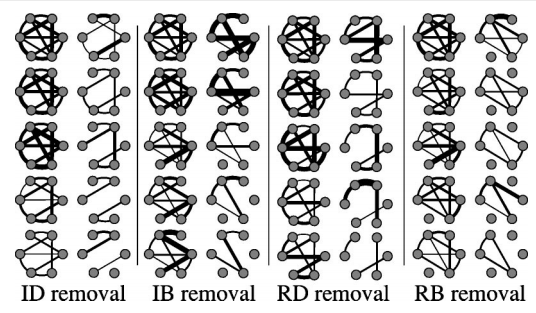
\includegraphics[width=0.5\textwidth]{edge_attacks.png}
	\caption{Various edge-centric attacks for a fixed graph topology.}
\end{figure}

RD and RB attacks on vertices yield the optimal results because they take a greedy approach to decrease the target metric. However, the implication of these attacks is that there exists an efficient and tractable way to measure these metrics after every change, which isn't always the case (especially when the topology of the network is unknown). Therefore, ID and IB attacks are more realistic, but they also assume some prior knowledge of the network infrastructure before the attack begins. Attacks that do not rely on this knowledge are referred to as random attacks, and are discussed in section~\ref{RandomFailures}.

Furthermore, it should be noted that both the ID and RD attacks are computationally less taxing than IB and RB attacks \cite{Attacks}. In fact, the time complexity of a successful ID attack (and subsequently, an entire RD attack), runs in linear time with respect to N, whereas the time complexity of betweenness-based attacks has a time complexity of $O(NL)$. The implication of this is that the adversary must make tradeoffs based on their knowledge of the network infrastructure.

\subsection{Random Failures}
\label{RandomFailures}
While targeted attacks model common scenarios in the real-world, it is often useful to disregard the source of and victim of such attacks and generalize the problem of network failures to encompass both random node and link failures. By doing so, we assume that each node and link has a fixed probability $p$ and $q$ of failing, where the exact cause of the failure is not know and is not important. Furthermore, failures are typically seen as independent events \cite{RandomStudy}. Such models are useful when analyzing complex networks such as the Internet and other related military communication networks. 

\section{Network Robustness}
%http://arxiv.org/pdf/1203.2982v1.pdf

Many different measures for network robustness have been proposed in recent years, all of which tend
to use the notion of densely connected components in the corresponding graph. 

%TODO: need more of an introduction here

\subsection{Robustness Measurements}

A natural way to think of network robustness is from the perspective of individual nodes, since they are 
usually the primary targets in malicious or non-malicious network attacks. Using this idea, Herrmann et al
defined a concise equation for calculating the robustness of a network based on the size of connected
components in the corresponding graph that is adapted from percolation theory. Mathematically, this can be defined as follows \cite{Onion}:
%24: http://polymer.bu.edu/~hes/networks/hsmah11.pdf
\begin{eqnarray*}
R_{n} = \frac{1}{n}\sum_{q=\frac{1}{n}}^{1}S(q)
\end{eqnarray*}
This robustness measurement computes the fractions of nodes in the largest connected cluster $S(q)$ after removing $q$ nodes. This is an intuitive calculation, since the goal of engineering robust networks is to ensure the highest measure of connectivity in the event of any node deletions. Furthermore, it has been mathematically verified to represent the exact amount of nodes that need to be deleted for the network to collapse when targeted by high-degree adaptive attacks, which are a specific class of attacks that attempt to remove highly connected nodes from the network. 

%TODO: http://arxiv.org/pdf/1203.2982v1.pdf, \cite{NRMalicious}

Another way to study the measure of robustness of a network is to examine its communication links. From the perspective of such links that exist in a network, the most successful attacks are those that take down the take down the most important or centralized communication links. As such, a common research trend has been to examine the largest components of a network with respect to the edge-betweenness, link clustering coefficient, and degree product \cite{NRMalicious}. One common measurement of the robustness of a network with respect to these metrics and the largest component of a network $S(p)$ is shown below:
\begin{eqnarray*}
R_l = \frac{1}{M}\sum_{p = 1/M}^{1}S(p)
\end{eqnarray*}
This measurement is mathematically similar to the previous node-based calculation, but instead of considering the density of the nodes in the entire component, it considers the density of the edges. 

Due to the typical attacks that are launched on networks, such as large-scale DDoS attacks that take both nodes and links to that node offline, it is natural to extend the concept of network robustness to consider both node and link failures simultaneously. However, rather because the two aforementioned measurements are based on two separate dimensions of networks, it is not simply a matter of merging them together to yield the optimum result. Instead, the measurement is typically abstracted into the context of the attack that is launched on a network, where the input parameter into the largest component is now the number of steps that have been completed at a given instance in time. Mathematically, this hybrid measurement $Q$ can be computed as follows \cite{NRMalicious}:
\begin{eqnarray*}
Q = \frac{1}{M}\sum_{step  = 1}^{M}S(step)
\end{eqnarray*}

\section{Random Graph Topologies}
% look at: http://web.mit.edu/medard/www/rls.pdf ???

%\subsection{Types of Random Graphs}
%There are many different models of random graphs that can be used to model real-world networks, %including the Erd\H{o}s

\subsection{Erd\"{o}s-R\`{e}nyi Graphs}
Erd\"{o}s-R\`{e}nyi graphs are the most simple random graphs that are defined by assigning a probabilistic uniform random variable to each edge. In other words, for each vertex $u, v \in V(G)$, where $G$ is a Erd\"{o}s-R\`{e}nyi graph, the edge $(u,v)$ exists in $E(G)$ with probability $p$, where $p$ is derived from a uniform random distribution, and each edge probability $p$ is independnt from the rest \cite{LargeNetworkRobustness-PVM}. When simulated using computers, it is not uncommon to derive the edge probabilities $p$ from an exponential distribution, due to its simplicity and similarity with the real-world. Another important element of these graphs is that they tend to have Poisson degree distributions, simply due to the random construction nature of the graph \cite{bimodal}.

%TODO: add a bit more about this.

\subsection{Scale-Free Graphs}
Scale-free graphs are special types of random graphs in that the distribution of node degrees $\langle k \rangle$ asymptotically follows a power law (i.e. $P(k) \approx k^{-\gamma})$. Many real-world networks have been found to have structures similar to scale-free graphs, so they are naturally used as the basis for random graph analysis \cite{AttacksWavesRandom}. 

%TODO: add a bit more about this.

\subsection{Graphs with Bimodal Degree Distribution}
%TODO: http://www.springerlink.com/content/3621163544501342/fulltext.pdf

Given the average degree $k$ for a graph $G = (V,E)$, we say that a graph has a bimodal degree distribution if its nodes fall under one of two categories \cite{bimodal}:
\begin{itemize}
	\item The local mean degree ($k_{loc}$) of a vertex $v$ is greater than the average degree distribution. That is, $k_{loc} > k$ for small. Such vertices are often referred to as "super-peers".
	\item The local mean degree ($k_{loc}$) of a vertex $v$ is less than or equal to the average degree distribution. That is, $k_{loc} \leq k$ for small. Such vertices are often referred to as "peers".
\end{itemize}
It is interesting to note that as the number of vertex modes or categories for a graph goes from $2$ to $\infty$, the degree distribution among all vertices in the graphs, and the hierarchy of peers in the graph, will begin to resemble that of a scale-free graph. Therefore, one can think of bimodal graphs as a special case of scale-free graphs that are useful when the power-law nature of the degree distribution complicates analytical efforts.

\section{Robustness Optimization}

Due to the complexity that exists in the aforementioned random graphs, most optimization algorithms utilize some large-scale stochastic process (similar to a Monte Carlo simulation) to randomly make changes to graph topology and test its measure of robustness. The exact measurement that is used depends on the type of experiements or simulations being performed. In this section, we discuss a sample of such efforts and the results that were found.

\subsection{Random and Scale-Free Graph Investigations}

%Assume that channel links have equal weight (that is, equal quality metrics, as described in functionality section)

Following the insight that hostile vertex attacks that target important nodes with large degrees tend to cause the most significant damage to a network, Albert et al. performed extensive studies on the robustness of random and scale-free graphs. 

By examining each of these classes of graphs in the context of random vertex deletions and targeted vertex attacks, it has been shown that random graphs are more robust against intentional vertex attacks, whereas the scale-free graphs are more robust against random deletions. This can be seen in Figure \ref{RandomResults}, where the breaking point of the largest component of the graphs $S$ drops off quicker for random graphs when attacked randomly \cite{GraphThesis}. 

\begin{figure}[h!]
	\label{fig:RandomResults}
	\centering
		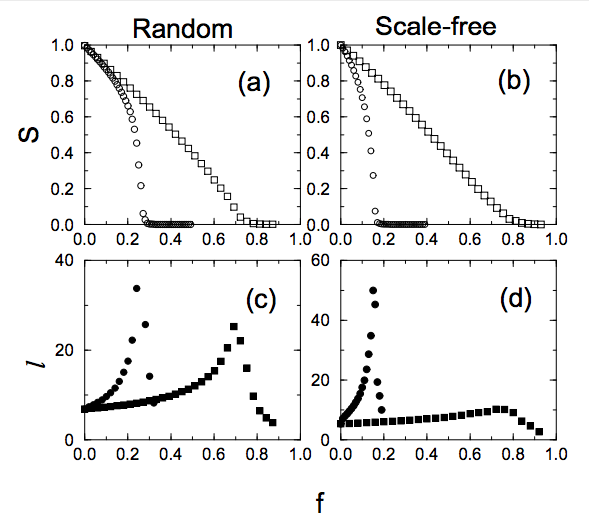
\includegraphics[width=0.5\textwidth]{random_results.png}
	\caption{Results of the random and scale-free graphs varied as $f$, the fraction of nodes removed from each graph, is changed . } %\cite{GraphThesis}
\end{figure}

\subsection{Fractional Node Deletion Investigations}

Finally, we introduce a metric that characterizes the number of nodes (or rather, a fraction of the total nodes) that need to be removed in order for the graph to become globally disconnected. Let $G$ be a graph with $N - q$ nodes of degree $1$. Then, the fraction of total nodes $f_c$ that need to be randomly removed before total connectivity is lost consists of $q = [(\langle k \rangle - 1) / \sqrt{\langle k \rangle}]\sqrt{N}$ nodes of degree $\sqrt{\langle k \rangle N}$. 

Paul et al. studied the robustness of random graphs in the context of random node deletions. Their work was driven by Monte Carlo simulations that approximated the fraction of nodes $f_c$ that would need to be removed from random networks in order for the graph to become globally disconnected. Formally, $f_c$ can be defined as in terms of the number of "hub" nodes that must be removed $q$ follows:
\begin{eqnarray*}
q = \left[(\langle k \rangle - 1) / \sqrt{\langle k \rangle}\right]\sqrt{N},
\end{eqnarray*}
where each of these vertices have degree $\sqrt{\langle k \rangle N}$ \cite{asd}. Thus, for a graph with $G = (V,E)$ with $N$ vertices, $q$ "hubs" would need to be removed in order to make $G$ disconnected, and thus $f_c = q/N$.

In terms of the design of a network, it is clear that network designers should strive for values of $q$ that imply high measures of robustness. Such a value of $q$ was determine empirically using a special degree distribution $P(k)$ that represents a network of $q$ hub nodes and $N-q$ leaf nodes, since this is a very general structure for such graphs. The simulation algorithm that was utilized to perform this caluclation is shown in Algorithm \ref{alg1} \cite{asd}. %http://polymer.bu.edu/hes/articles/pshs06.pdf 

\begin{numberedAlg}[Monte-Carlo $q$ Determination]
\label{alg1}
\begin{algorithmic}[1]
        \item Initialize a graph $G$ with $N$ vertices.
	\item Randomly delete a node in the network and calculate $\kappa(G)$.
	\item Increment $q$ by 1 node.
	\item If $\kappa < 2$, $G$ has become disconnected, so terminate and return $q$. Otherwise, decrement $q$ by 1 and go to step 2.
\end{algorithmic}
\end{numberedAlg}

\begin{figure}[h!]
	\label{fig:Onion}
	\centering
		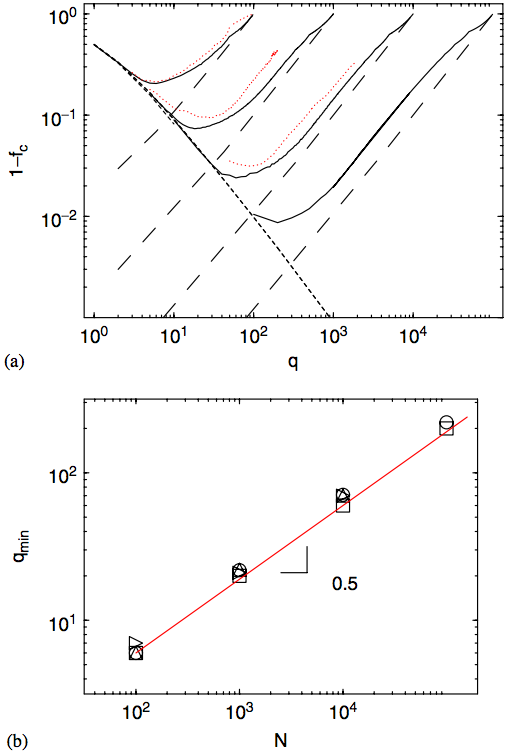
\includegraphics[width=0.5\textwidth]{fractional_results.png}
	\caption{TODO}
\end{figure}

%TODO: read http://polymer.bu.edu/hes/articles/pshs06.pdf and discuss the metric here - devote entire section to it in the NR part

\subsection{Fixed-Degree Distribution Investigations}

%TODO: the work was done independently

In their study of optimal graph structures that yield the highest resilience to such attacks, Herrmann et al found that most networks will exhibit onion topolgies, meaning that there are distinct layers of nodes that are connected, and that each layer $i$ has more connectivity than its parent layer $i+1$ \cite{Onion}. Another interesting property of the onion graph is that for almost every pair of vertices $u, v \in V(G)$ with the same degree, there exists a a path between $u$ and $v$ that does not contain any vertex of a higher degree. An example of such a graph with $124$ nodes and $366$ edges is shown in Figure~\ref{fig:Onion}.

\begin{figure}[h!]
	\label{fig:Onion}
	\centering
		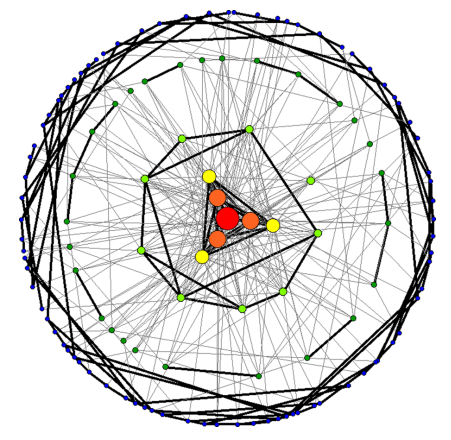
\includegraphics[width=0.5\textwidth]{Onion.jpg}
	\caption{An example of a graph with $124$ nodes and $366$ edges that exhibits the onion-like topology } %\cite{Onion}
\end{figure}

Herrmann et al have also conducted research on optimization algorithms that increase this robustness measure while at the same time maintaining the distribution of vertex degrees throughout the network. Their proposed algorithm seeks to re-arrange node edges and connections to improve the resilience of the host network to any kinds of attacks using Monte-Carlo simulations. This algorithm can be described as follows:

% the re-structure algorithm
\begin{numberedAlg}[Robustness Optimization]
\label{alg2}
\begin{algorithmic}[1]
        \item Choose two random edges $(a,b)$ and $(c,d)$ from the graph $G$.
	\item Replace these edges with $(a,c)$ and $(b,d)$.
	\item If $R_{new} > R_{old}$, accept the swap and go to step 1. Otherwise, revert the swap and goto step 1. 
\end{algorithmic}
\end{numberedAlg}

Algorithm~\ref{alg2} is repeated for a very large number of iterations until an ideal level of robustness has been obtained, albiet at the sake of sometimes massive computations (as is the case with Monte-Carlo methods).

%%%%%%%%%% Bimodal discussion, how they simulated and concluded that bimodal was the best

One more recent investigation of graphs with fixed degree distributions was performed by Sonawane et al \cite{bimodal}. 

% Here is the bibliography
%\bibliographystyle{plain}
\bibliography{nr}

% That's all folks
\end{document}
